\chapter{Introduzione}\label{cap:introduzione}

\intro{Il seguente capitolo vuole introdurre brevemente l'azienda con il relativo contesto aziendale e l'organizzazione del testo con le norme tipografiche adottate.}\\

\section{L'azienda}\label{sec:azienda}
THRON S.p.A è un'azienda italiana con sede a Piazzola sul Brenta specializzata nello sviluppo di \textit{SaaS} (\textit{Software as a Service}).
I suoi prodotti principali sono la \textit{THRON DAM Platform} e il \textit{THRON PIM}~\cite{site:thron}. 
Il primo è una piattaforma nata con l'obiettivo di gestire, organizzare e distribuire i contenuti digitali di un'azienda (riferimenti in~\cite{site:dam}).
Il \textit{THRON PIM} invece è una soluzione per la gestione delle informazioni sui prodotti, che si concentra
sulla raccolta, organizzazione e distribuzione delle informazioni relative ai prodotti di un'azienda (riferimenti in~\cite{site:pim}).\\
In sintesi, il primo prodotto si concentra sulla gestione dei contenuti digitali, il secondo invece
si focalizza sulla gestione delle informazioni sui prodotti.
L'obiettivo è garantire una gestione centralizzata dei contenuti e semplificarne l'adattamento e la distribuzione su diversi
canali in modo efficiente.
All'interno dell'azienda, l'area \textit{R\&D} è suddivisa in due team: il team Prodotti, responsabile della gestione
del \glsfirstoccur{\gls{pimg}}, e il team Contenuti, focalizzato sulle tematiche legate al \glsfirstoccur{\gls{damg}}.\\
Durante il mio stage presso l'azienda, sono stato inserito come sviluppatore \glsfirstoccur{\gls{frontendg}} all'interno dell'area Prodotto, nel team Prodotti.

\section{Metodologie di sviluppo}\label{sec:metodologie-sviluppo}
Nel contesto aziendale di THRON, vengono adottate metodologie di sviluppo \glsfirstoccur{\gls{agileg}} per garantire un'efficace
gestione dei progetti. La filosofia \textit{Agile} pone un forte \textit{focus} sulla collaborazione tra i membri del team,
sulla capacità di rispondere in modo rapido ai cambiamenti, nonchè sull'orientamento al cliente e alla consegna di prodotti qualitativi (riferimenti in~\cite{site:agile-manifesto}).\\
Il \glsfirstoccur{\gls{frameworkg}} \glsfirstoccur{\gls{scrumg}}  parte integrante dell'approccio \textit{Agile}, è utilizzato all'interno dell'azienda per organizzare il lavoro in iterazioni chiamate
\glsfirstoccur{\gls{sprintg}} della durata di due settimane ciascuna. Questo approccio a breve termine consente al team di concentrarsi su attività specifiche, pianificando
e completando le attività in maniera incrementale.\\
Al termine di ogni \textit{Sprint} vengono organizzate molteplici riunioni: `\textit{Sprint Review}', in cui il team presenta i risultati ottenuti durante lo \textit{Sprint},
`\textit{Sprint Planning}', in cui vengono pianificate le attività da svolgere durante lo \textit{Sprint} successivo e `\textit{Sprint Retrospective}', in cui il team riflette sulle prestazioni del team e sulle possibili migliorie.\\
L'importanza della comunicazione e della condivisione delle informazioni è supportata dalla pratica quotidiana della riunione `\textit{Daily Scrum}', durante la quale
ogni membro del team esprime il proprio progresso, eventuali ostacoli e le prossime attività pianificate. Questa pratica aiuta a mantenere l'allineamento e
la trasparenza, nonché a individuare tempestivamente eventuali problemi da risolvere (riferimenti in~\cite{site:scrum}).\\
Le riunioni settimanali chiamate `\textit{Competence}' rappresentano un'altra componente importante adottata da THRON. Riunendo i membri dello sviluppo 
che condividono la stessa area di competenza, come frontend o \glsfirstoccur{\gls{backendg}}, queste riunioni offrono un'opportunità di scambio di conoscenze e di valutazione dei progressi.
\section{Strumenti di sviluppo}\label{sec:strumenti-sviluppo}
Durante l'esperienza di stage presso THRON, l'utilizzo di una varietà di strumenti di sviluppo è stato fondamentale per assicurare un processo di lavoro efficiente.\\
Di seguito, sono elencati gli strumenti che sono stati impiegati per lo sviluppo del progetto:

\begin{itemize}
  \item \textbf{\textit{Teams}}: per le comunicazione sia asincrone che sincrone con il team;
  \item \textbf{\textit{Microsoft 365}} per la gestione della mail aziendale~\cite{site:microsoft365};
  \item \textbf{\textit{Jira}} per il tracciamento e la gestione delle attività assegnate durante il periodo di stage (esempio in figura~\ref{fig:board-jira})~\cite{site:jira};
  \item \textbf{\textit{AWS}} per la gestione della \glsfirstoccur{\gls{repositoryg}} del mio progetto, per la \glsfirstoccur{\gls{buildg}} e per il \glsfirstoccur{\gls{deployg}} dello stesso~\cite{site:aws};
  \item \textbf{\textit{Fork}} per la gestione del versionamento del codice sorgente~\cite{site:fork};
  \item \textbf{\textit{Postman}} per la creazione, esecuzione e test delle chiamate verso gli \glsfirstoccur{\gls{endpointg}} creati durante lo sviluppo~\cite{site:postman};
  \item \textbf{\textit{Confluence}} per la creazione e gestione della documentazione relativa al progetto di stage~\cite{site:confluence};
  \item \textbf{\textit{StarUML}} per la modellazione dei casi d'uso~\cite{site:staruml}.
\end{itemize}

\begin{figure}[!ht] 
  \centering 
  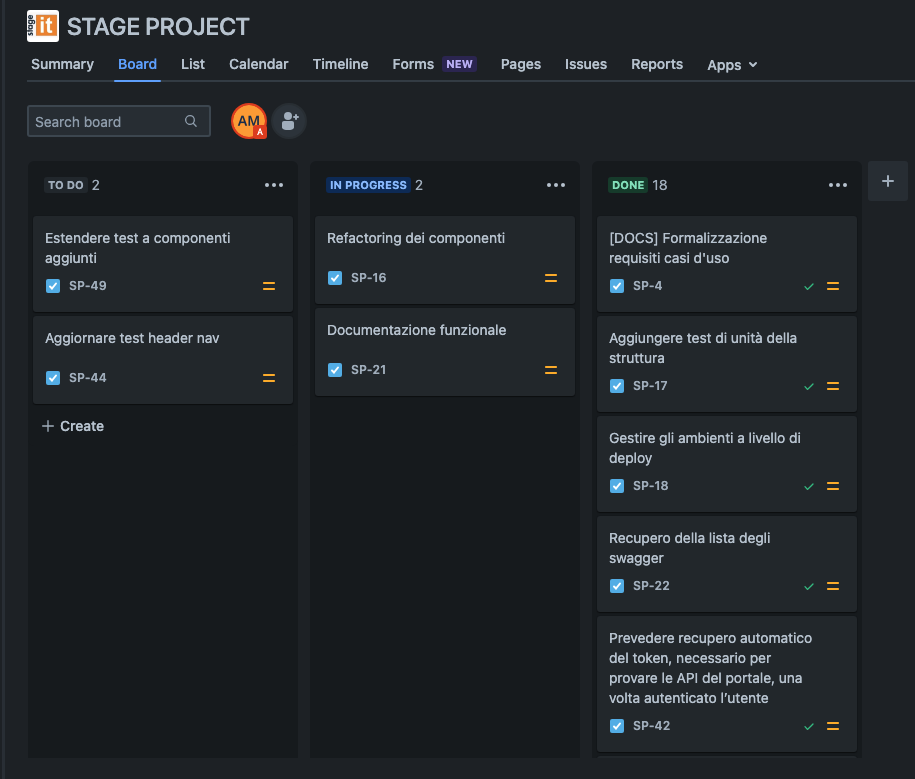
\includegraphics[width=0.9\columnwidth, alt={Esempio di utilizzo della board di Jira}]{images/Board.jpg}
  \caption{Board Jira}\label{fig:board-jira}
\end{figure}

\section{Organizzazione del testo}\label{sec:organizzazione-testo}
\begin{description}
    \item[{\hyperref[cap:descrizione-stage]{Il secondo capitolo}}] descrive il progetto svolto durante il periodo di stage, mettendo in risalto gli obiettivi imposti dall'azienda e i possibili rischi.
    \item[{\hyperref[cap:analisi-requisiti]{Il terzo capitolo}}] descrive l'analisi dei requisiti del progetto di stage attraverso la modellazione dei casi d'uso e l'estrapolazione dei requisiti partendo da essi.
    \item[{\hyperref[cap:struttura-progettazione]{Il quarto capitolo}}] approfondisce le tecnologie utilizzate per lo sviluppo del progetto, introduce la sua struttura principale e descrive le scelte progettuali effettuate.
    \item[{\hyperref[cap:codifica]{Il quinto capitolo}}] descrive le attività di codifica effettuate durante lo stage, dividendole tra frontend e backend.
    \item[{\hyperref[cap:verifica-validazione]{Il sesto capitolo}}] descrive le attività di verifica e validazione, descrivendo i test effettuati e i risultati ottenuti.
    \item[{\hyperref[cap:conclusioni]{Il settimo capitolo}}] presenta le conclusioni tratte dallo stage, esponendo le conoscenze acquisite, le competenze sviluppate e le considerazioni personali. 
\end{description}

\clearpage

Per quanto riguarda la formattazione del testo nel documento, sono state seguite le seguenti convenzioni tipografiche:
\begin{itemize}
  \item Le abbreviazioni, gli acronimi e i termini poco comuni menzionati sono definiti nel glossario, situato alla fine del seguente documento;
  \item I termini in lingua straniera o appartenenti al gergo tecnico sono evidenziati utilizzando il carattere corsivo;
  \item Ogni termine presente nel glossario, è contrassegnato dalla lettera `G' come apice.
\end{itemize}
